\documentclass[a4paper]{article}

% --- Packages ---

\usepackage{a4wide}
\usepackage[utf8]{inputenc}
\usepackage{amsmath}
\usepackage{mathtools}
\usepackage{amssymb}
\usepackage[english]{babel}
\usepackage{mdframed}
\usepackage{systeme,}
\usepackage{lipsum}
\usepackage{relsize}
\usepackage{caption}
\usepackage{tikz}
\usepackage{tikz-3dplot}
\usetikzlibrary{shapes.geometric}
\usepackage{pgfplots}
\usepackage{pgfplotstable}
\pgfplotsset{compat=newest}%1.7}
\usepackage{harpoon}%
\usepackage{graphicx}
\usepackage{wrapfig}
\usepackage{subcaption}
\usepackage{authblk}
\usepackage{float}
\usepackage{listings}
\usepackage{xcolor}
\usepackage{chngcntr}
\usepackage{amsthm}
\usepackage{comment}
\usepackage{commath}
\usepackage{hyperref}%Might remove, adds link to each reference
\usepackage{url}
\usepackage{calligra}
\usepackage{pgf}

% --- Bibtex ---

%\usepackage[backend = biblar,]{bibtex}

%\addbibliografy(ref.bib)

% --- Commands --- 

\newcommand{\w}{\omega}
\newcommand{\trace}{\text{Tr}}
\newcommand{\grad}{\mathbf{\nabla}}
%\newcommand{\crr}{\mathfrak{r}}
\newcommand{\laplace}{\nabla^2}
\newcommand{\newparagraph}{\vspace{.5cm}\noindent}

% --- Math character commands ---

\newcommand{\curl}[1]{\mathbf{\nabla}\times \mathbf{#1}}
\newcommand{\dive}[1]{\mathbf{\nabla}\cdot \mathbf{#1}}
\newcommand{\res}[2]{\text{Res}(#1,#2)}
\newcommand{\fpartial}[2]{\frac{\partial #1}{\partial #2}}
\newcommand{\rot}[3]{\begin{vmatrix}\hat{x}&\hat{y}&\hat{z}\\\partial_x&\partial_y&\partial_z\\#1&#2&#3 \end{vmatrix}}
\newcommand{\average}[1]{\langle #1 \rangle}
\newcommand{\ket}[1]{|#1\rangle}
\newcommand{\bra}[1]{\langle #1|}


%  --- Special character commands ---

\DeclareMathAlphabet{\mathcalligra}{T1}{calligra}{m}{n}
\DeclareFontShape{T1}{calligra}{m}{n}{<->s*[2.2]callig15}{}
\newcommand{\crr}{\mathcalligra{r}\,}
\newcommand{\boldscriptr}{\pmb{\mathcalligra{r}}\,}


\title{Handin 5}
\author{Author : Andreas Evensen}
\date{Date: \today}

% --- Code ---

\definecolor{codegreen}{rgb}{0,0.6,0}
\definecolor{codegray}{rgb}{0.5,0.5,0.5}
\definecolor{codepurple}{rgb}{0.58,0,0.82}
\definecolor{backcolour}{rgb}{0.95,0.95,0.92}

\lstdefinestyle{mystyle}{
    backgroundcolor=\color{backcolour},   
    commentstyle=\color{codegreen},
    keywordstyle=\color{magenta},
    numberstyle=\tiny\color{codegray},
    stringstyle=\color{codepurple},
    basicstyle=\ttfamily\footnotesize,
    breakatwhitespace=false,         
    breaklines=true,                 
    captionpos=b,                    
    keepspaces=true,                 
    numbers=left,                    
    numbersep=5pt,                  
    showspaces=false,                
    showstringspaces=false,
    showtabs=false,                  
    tabsize=2
}

\lstset{style=mystyle}

\begin{document}

\maketitle

\subsection*{Question 1}
\begin{comment}
We have the following probability distribution:
\begin{figure}[H]
    \centering
    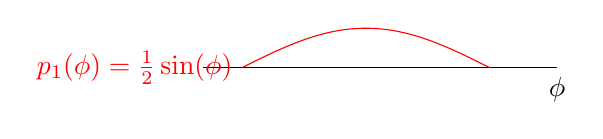
\begin{tikzpicture}
        \draw (-0.5,0) -- (4, 0) node[below] {$\phi$};
        \draw[color = red] plot[domain = 0:pi, samples = 100] (\x, {1/2 * sin(\x r)}) node[left, pos = 0.5] {$p_1(\phi)=\frac{1}{2}\sin(\phi)$};
    \end{tikzpicture}
    \caption{Probability distribution 1}
\end{figure}\noindent
We do this by finding:
\begin{align*}
    u(\phi) &= \int_{\phi_0}^\phi p_1(\phi')d{\phi'}\\
    &= \int_{\phi_0}^\phi \frac{1}{2}\sin(\phi')d{\phi'}\\
    &= -\frac{1}{2}\cos(\phi')\Big|_{\phi_0}^\phi\\
    &= \frac{1}{2}\left(\cos(\phi_0) - \cos(\phi)\right).
\end{align*}We now want to find the inverse of $u(\phi)$, which is given by:
\begin{align*}
    2u &= \cos(\phi_0) - \cos(\phi)\\
    \cos(\phi) &= \cos(\phi_0) - 2u\\
    \phi &= \arccos(\cos(\phi_0) - 2u).
\end{align*}Thus, any random number $u$ describes a random value $\phi$. 
\end{comment}
Say that we have a uniform probability distribution for values of $x\in[0,1]$.
We want to transform such a distribution to a distribution for $\pi\in[0, \pi]$, such that the probability distribution is given by $p_1(\phi) = \frac{1}{2}\sin(\phi)$.
We can do this by using the method of importance sampling.
One have that the probability distribution for $x$ is given by $p_0(x) = 1$.
Then we can find the probability distribution for $\phi$ by using the following relation:
\begin{align*}
    p_1(\phi) &= p_0(x)\abs{\frac{dx}{d\phi}}\\
    &= \abs{\frac{dx}{d\phi}}.
\end{align*}We can find the relation between $x$ and $\phi$ by integrating the probability distribution $p_1(\phi)$:
\begin{align*}
    u(\phi) &= \int_{\phi_0}^\phi p_1(\phi')d{\phi'}\\
    &= \int_{\phi_0}^\phi \frac{1}{2}\sin(\phi')d{\phi'}\\
    &= -\frac{1}{2}\cos(\phi')\Big|_{\phi_0}^\phi\\
    &= \frac{1}{2}\left(\cos(\phi_0) - \cos(\phi)\right).
\end{align*}We now want to find the inverse of $u(\phi)$, which is given by:
\begin{align*}
    2u &= \cos(\phi_0) - \cos(\phi)\\
    \cos(\phi) &= \cos(\phi_0) - 2u\\
    \phi &= \arccos(\cos(\phi_0) - 2u).
\end{align*}Thus, any random number $u$ describes a random value $\phi$.
\begin{figure}[H]
    \centering
    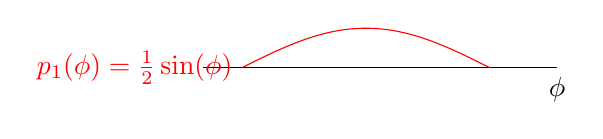
\begin{tikzpicture}
        \draw (-0.5,0) -- (4, 0) node[below] {$\phi$};
        \draw[color = red] plot[domain = 0:pi, samples = 100] (\x, {1/2 * sin(\x r)}) node[left, pos = 0.5] {$p_1(\phi)=\frac{1}{2}\sin(\phi)$};
    \end{tikzpicture}
    \caption{Probability distribution 1}
\end{figure}\noindent



\subsection*{Question 2}

The method of importance sampling is a method to sample from a probability distribution $p(x)$, by sampling from a different distribution $q(x)$, which is easier to sample from.
The idea is to sample from $q(x)$, and then use the samples to estimate the expectation value of some function $f(x)$ with respect to $p(x)$.
We do this by looking at the integral of the approximated probability distribution, as the slope of the integrated function is proportional to the probability distribution.

\begin{figure}[H]
    \centering
    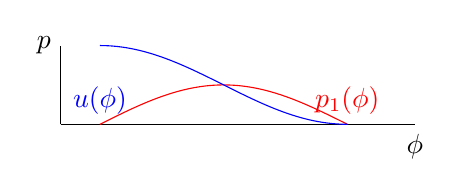
\begin{tikzpicture}
        \draw(-0.5,0) -- (4,0) node[below] {$\phi$};
        \draw(-.5, 0) -- (-.5, 1) node[left] {$p$};
        \draw[color = red] plot[domain = 0:pi, samples = 100] (\x, {1/2 * sin(\x r)}) node[above] {$p_1(\phi)$};
        \draw[color = blue] plot[domain = 0:pi, samples = 100] (\x, {1/2 * cos(\x r) + 1/2}) node[above, pos = 0.5] {$u(\phi)$};
    \end{tikzpicture}
    \caption{$p_1(\phi)$ and $u(\phi)$}
\end{figure}\noindent
We can in the above figure see that the probability slope of the integrated function $u(\phi)$ is proportional to the probability distribution $p_1(\phi)$.

\subsection*{Question 3}
Now suppose $p_2(\phi) = \frac{1}{2}\sin^2(\phi)$. We wish to sample the $p_2(\phi)$ distribution based on random number obtained by $p_1(\phi)$.
We can do this by using the method of importance sampling.
One has that the probability distribution for $p_2(\phi)$ is given by:
\begin{align*}
    p_2(\phi) &= p_1(\phi)\abs{\frac{du}{d\phi}}\\
    &= \frac{1}{2}\sin(\phi)\abs{\frac{du}{d\phi}}.
\end{align*}We can find the relation between $u$ and $\phi$ by integrating the probability distribution $p_2(\phi)$:
\begin{align*}
    v(\phi) &= \int_{\phi_0}^\phi p_2(\phi')d{\phi'}\\
    &= \int_{\phi_0}^\phi \frac{1}{2}\sin^2(\phi')d{\phi'}\\
    &= \frac{1}{4}\left(\phi - \sin(\phi)\cos(\phi)\right).
\end{align*}We now want to find the inverse of $v(\phi)$, which is given by:
\begin{align*}
    4v &= \phi - \sin(\phi)\cos(\phi)\\
    \phi &= \arcsin\left(\frac{4v}{\sqrt{16v^2 + 1}}\right).
\end{align*}Thus, any random number $v$ describes a random value $\phi$.

\subsection*{Question 4}
Suppose now, that instead we have a random uniform distribution $p_3(\phi) = \frac{1}{2}$.
How does one then obtain a random number $\phi_{rand}$?
We, have that the probability distribution for $p_3(\phi)$ is given by:
\begin{align*}
    p_3(\phi) &= p_1(\phi)\abs{\frac{du}{d\phi}}\\
    &= \frac{1}{2}\sin(\phi)\abs{\frac{du}{d\phi}}.
\end{align*}We can find the relation between $u$ and $\phi$ by integrating the probability distribution $p_3(\phi)$:
\begin{align*}
    w(\phi) &= \int_{\phi_0}^\phi p_3(\phi')d{\phi'}\\
    &= \int_{\phi_0}^\phi \frac{1}{2}d{\phi'}\\
    &= \frac{1}{2}\phi.
\end{align*}One now want to find the inverse of $w(\phi)$, which is given by:
\begin{align*}
    2u &= \phi\\
    \phi &= 2u.
\end{align*}Thus, any random number $u$ describes a random value $\phi$.
The efficiency of the last method is not as good as the previous method, one has to complete more samples to obtain a good estimate of the probability distribution; whereas the previous method requires fewer samples to obtain a good estimate of the probability distribution.

\end{document}
 
